% Submission manuscript for Cognition and Emotion (Brief Article). Requirements: docs/journal_target.md.
% Every result is generated by analysis/05_report_numbers.py (\val{key}); none is typed by hand.
% Items marked [AUTHOR TO CONFIRM] need information only the author can give.
% Build from this directory: latexmk -pdf manuscript.tex. Word count: uv run python analysis/08_word_count.py.
\documentclass[man,12pt,donotrepeattitle,british]{apa7}

\usepackage[british]{babel}
\usepackage[T1]{fontenc}
\usepackage{newtxtext,newtxmath} % Times-style; heavier strokes than Latin Modern, easier to read on screens
\usepackage{booktabs}
\usepackage{array}
\usepackage{graphicx}
\usepackage{amsmath}
\usepackage{csquotes}
\usepackage{xcolor}
\usepackage[style=apa,backend=biber]{biblatex}
\DeclareLanguageMapping{british}{british-apa}
\addbibresource{references.bib}
\graphicspath{{figures/}}

% Written by analysis/05_report_numbers.py - do not edit by hand.
\newcommand{\val}[1]{\ifcsname val:#1\endcsname\csname val:#1\endcsname\else\errmessage{Unknown value #1}\fi}
\expandafter\def\csname val:n_completed\endcsname{130}
\expandafter\def\csname val:n_excluded\endcsname{6}
\expandafter\def\csname val:n_primary\endcsname{124}
\expandafter\def\csname val:n_excl_disrupted\endcsname{3}
\expandafter\def\csname val:n_excl_freetext\endcsname{2}
\expandafter\def\csname val:n_excl_erratic\endcsname{1}
\expandafter\def\csname val:n_cohort_two\endcsname{19}
\expandafter\def\csname val:n_cohort_three\endcsname{20}
\expandafter\def\csname val:n_cohort_four\endcsname{85}
\expandafter\def\csname val:n_age\endcsname{121}
\expandafter\def\csname val:age_mean\endcsname{34.2}
\expandafter\def\csname val:age_sd\endcsname{12.0}
\expandafter\def\csname val:age_min\endcsname{18}
\expandafter\def\csname val:age_max\endcsname{76}
\expandafter\def\csname val:n_female\endcsname{59}
\expandafter\def\csname val:n_male\endcsname{62}
\expandafter\def\csname val:n_sex_missing\endcsname{3}
\expandafter\def\csname val:n_mouse\endcsname{80}
\expandafter\def\csname val:n_trackpad\endcsname{43}
\expandafter\def\csname val:n_stricter\endcsname{96}
\expandafter\def\csname val:n_sparse\endcsname{24}
\expandafter\def\csname val:n_one_check\endcsname{5}
\expandafter\def\csname val:n_not_attentive\endcsname{3}
\expandafter\def\csname val:n_without_rejected\endcsname{120}
\expandafter\def\csname val:n_rejection_set\endcsname{4}
\expandafter\def\csname val:n_exploratory_completed\endcsname{23}
\expandafter\def\csname val:n_exploratory\endcsname{21}
\expandafter\def\csname val:height_fear_mean\endcsname{3.77}
\expandafter\def\csname val:height_fear_sd\endcsname{1.73}
\expandafter\def\csname val:height_fear_median\endcsname{4}
\expandafter\def\csname val:sticsa_pre_mean\endcsname{13.76}
\expandafter\def\csname val:sticsa_pre_sd\endcsname{3.56}
\expandafter\def\csname val:sticsa_pre_median\endcsname{13}
\expandafter\def\csname val:sticsa_post_mean\endcsname{20.55}
\expandafter\def\csname val:sticsa_post_sd\endcsname{7.29}
\expandafter\def\csname val:sticsa_post_median\endcsname{18}
\expandafter\def\csname val:sticsa_change_mean\endcsname{6.79}
\expandafter\def\csname val:sticsa_change_sd\endcsname{6.60}
\expandafter\def\csname val:sticsa_change_median\endcsname{5}
\expandafter\def\csname val:anxiety_overall_mean\endcsname{5.18}
\expandafter\def\csname val:anxiety_overall_sd\endcsname{1.33}
\expandafter\def\csname val:anxiety_overall_median\endcsname{5}
\expandafter\def\csname val:concern_safety_mean\endcsname{6.13}
\expandafter\def\csname val:concern_safety_sd\endcsname{1.30}
\expandafter\def\csname val:concern_safety_median\endcsname{7}
\expandafter\def\csname val:body_intensity_mean\endcsname{4.64}
\expandafter\def\csname val:body_intensity_sd\endcsname{1.60}
\expandafter\def\csname val:body_intensity_median\endcsname{5}
\expandafter\def\csname val:arousal_baseline_mean\endcsname{43.13}
\expandafter\def\csname val:arousal_baseline_sd\endcsname{15.80}
\expandafter\def\csname val:arousal_baseline_median\endcsname{43.8}
\expandafter\def\csname val:arousal_rise_mean\endcsname{67.14}
\expandafter\def\csname val:arousal_rise_sd\endcsname{14.79}
\expandafter\def\csname val:arousal_rise_median\endcsname{68.9}
\expandafter\def\csname val:arousal_plateau_mean\endcsname{80.91}
\expandafter\def\csname val:arousal_plateau_sd\endcsname{15.01}
\expandafter\def\csname val:arousal_plateau_median\endcsname{83.1}
\expandafter\def\csname val:arousal_return_mean\endcsname{53.89}
\expandafter\def\csname val:arousal_return_sd\endcsname{19.42}
\expandafter\def\csname val:arousal_return_median\endcsname{54.8}
\expandafter\def\csname val:arousal_whole_film_mean\endcsname{61.23}
\expandafter\def\csname val:arousal_whole_film_sd\endcsname{10.99}
\expandafter\def\csname val:arousal_whole_film_median\endcsname{60.6}
\expandafter\def\csname val:valence_baseline_mean\endcsname{50.58}
\expandafter\def\csname val:valence_baseline_sd\endcsname{14.55}
\expandafter\def\csname val:valence_baseline_median\endcsname{52.0}
\expandafter\def\csname val:valence_rise_mean\endcsname{39.58}
\expandafter\def\csname val:valence_rise_sd\endcsname{19.06}
\expandafter\def\csname val:valence_rise_median\endcsname{38.5}
\expandafter\def\csname val:valence_plateau_mean\endcsname{29.13}
\expandafter\def\csname val:valence_plateau_sd\endcsname{23.10}
\expandafter\def\csname val:valence_plateau_median\endcsname{23.9}
\expandafter\def\csname val:valence_return_mean\endcsname{50.84}
\expandafter\def\csname val:valence_return_sd\endcsname{20.44}
\expandafter\def\csname val:valence_return_median\endcsname{51.7}
\expandafter\def\csname val:valence_whole_film_mean\endcsname{41.89}
\expandafter\def\csname val:valence_whole_film_sd\endcsname{14.67}
\expandafter\def\csname val:valence_whole_film_median\endcsname{41.9}
\expandafter\def\csname val:H1:report\endcsname{$t$(123) = 11.46, $p$ < .001, $d_z$ = 1.03, 95\% CI [0.81, 1.25]}
\expandafter\def\csname val:H1:effect\endcsname{$d_z$ = 1.03 [0.81, 1.25]}
\expandafter\def\csname val:H1:est\endcsname{1.03}
\expandafter\def\csname val:H1:diff\endcsname{6.79}
\expandafter\def\csname val:H1:diffabs\endcsname{6.79}
\expandafter\def\csname val:H2a:report\endcsname{$t$(123) = 14.67, $p_\mathrm{Holm}$ < .001, $d_z$ = 1.32, 95\% CI [1.07, 1.56]}
\expandafter\def\csname val:H2a:effect\endcsname{$d_z$ = 1.32 [1.07, 1.56]}
\expandafter\def\csname val:H2a:est\endcsname{1.32}
\expandafter\def\csname val:H2a:diff\endcsname{24.01}
\expandafter\def\csname val:H2a:diffabs\endcsname{24.01}
\expandafter\def\csname val:H2b:report\endcsname{$t$(123) = 19.77, $p_\mathrm{Holm}$ < .001, $d_z$ = 1.78, 95\% CI [1.49, 2.06]}
\expandafter\def\csname val:H2b:effect\endcsname{$d_z$ = 1.78 [1.49, 2.06]}
\expandafter\def\csname val:H2b:est\endcsname{1.78}
\expandafter\def\csname val:H2b:diff\endcsname{37.78}
\expandafter\def\csname val:H2b:diffabs\endcsname{37.78}
\expandafter\def\csname val:H2c:report\endcsname{$t$(123) = $-$14.70, $p_\mathrm{Holm}$ < .001, $d_z$ = $-$1.32, 95\% CI [$-$1.56, $-$1.08]}
\expandafter\def\csname val:H2c:effect\endcsname{$d_z$ = $-$1.32 [$-$1.56, $-$1.08]}
\expandafter\def\csname val:H2c:est\endcsname{$-$1.32}
\expandafter\def\csname val:H2c:diff\endcsname{$-$27.02}
\expandafter\def\csname val:H2c:diffabs\endcsname{27.02}
\expandafter\def\csname val:H2d:report\endcsname{$t$(123) = $-$9.85, $p_\mathrm{Holm}$ < .001, $d_z$ = $-$0.88, 95\% CI [$-$1.09, $-$0.68]}
\expandafter\def\csname val:H2d:effect\endcsname{$d_z$ = $-$0.88 [$-$1.09, $-$0.68]}
\expandafter\def\csname val:H2d:est\endcsname{$-$0.88}
\expandafter\def\csname val:H2d:diff\endcsname{$-$21.44}
\expandafter\def\csname val:H2d:diffabs\endcsname{21.44}
\expandafter\def\csname val:H3arousal:report\endcsname{$r$ = .993, 95\% CI [.990, .996]}
\expandafter\def\csname val:H3arousal:effect\endcsname{$r$ = .993 [.990, .996]}
\expandafter\def\csname val:H3arousal:est\endcsname{.99}
\expandafter\def\csname val:H3valence:report\endcsname{$r$ = .937, 95\% CI [.893, .966]}
\expandafter\def\csname val:H3valence:effect\endcsname{$r$ = .937 [.893, .966]}
\expandafter\def\csname val:H3valence:est\endcsname{.94}
\expandafter\def\csname val:H4a:report\endcsname{$\rho$ = .08, 95\% CI [$-$.09, .26], $p$ = .355, $p_\mathrm{Holm}$ = .355}
\expandafter\def\csname val:H4a:effect\endcsname{$\rho$ = .08 [$-$.09, .26]}
\expandafter\def\csname val:H4a:est\endcsname{.08}
\expandafter\def\csname val:H4b:report\endcsname{$\rho$ = $-$.32, 95\% CI [$-$.46, $-$.16], $p$ < .001, $p_\mathrm{Holm}$ = .001}
\expandafter\def\csname val:H4b:effect\endcsname{$\rho$ = $-$.32 [$-$.46, $-$.16]}
\expandafter\def\csname val:H4b:est\endcsname{$-$.32}
\expandafter\def\csname val:H4c:report\endcsname{$\rho$ = .18, 95\% CI [.00, .35], $p$ = .049, $p_\mathrm{Holm}$ = .098}
\expandafter\def\csname val:H4c:effect\endcsname{$\rho$ = .18 [.00, .35]}
\expandafter\def\csname val:H4c:est\endcsname{.18}
\expandafter\def\csname val:H5a:report\endcsname{$\rho$ = .24, 95\% CI [.05, .41], $p$ = .008, $p_\mathrm{Holm}$ = .008}
\expandafter\def\csname val:H5a:effect\endcsname{$\rho$ = .24 [.05, .41]}
\expandafter\def\csname val:H5a:est\endcsname{.24}
\expandafter\def\csname val:H5b:report\endcsname{$\rho$ = $-$.38, 95\% CI [$-$.51, $-$.23], $p$ < .001, $p_\mathrm{Holm}$ < .001}
\expandafter\def\csname val:H5b:effect\endcsname{$\rho$ = $-$.38 [$-$.51, $-$.23]}
\expandafter\def\csname val:H5b:est\endcsname{$-$.38}
\expandafter\def\csname val:H6a:report\endcsname{$\rho$ = .56, 95\% CI [.44, .67], $p$ < .001, $p_\mathrm{Holm}$ < .001}
\expandafter\def\csname val:H6a:effect\endcsname{$\rho$ = .56 [.44, .67]}
\expandafter\def\csname val:H6a:est\endcsname{.56}
\expandafter\def\csname val:H6b:report\endcsname{$\rho$ = .34, 95\% CI [.15, .50], $p$ < .001, $p_\mathrm{Holm}$ < .001}
\expandafter\def\csname val:H6b:effect\endcsname{$\rho$ = .34 [.15, .50]}
\expandafter\def\csname val:H6b:est\endcsname{.34}
\expandafter\def\csname val:H2:absrange\endcsname{0.88--1.78}
\expandafter\def\csname val:H1:wilcoxon\endcsname{$T$ = 197, $p$ < .001}
\expandafter\def\csname val:n_floor_pre\endcsname{45}
\expandafter\def\csname val:pct_floor_pre\endcsname{36}
\expandafter\def\csname val:n_increase\endcsname{109}
\expandafter\def\csname val:n_nochange\endcsname{7}
\expandafter\def\csname val:n_decrease\endcsname{8}
\expandafter\def\csname val:n_fear_top\endcsname{20}
\expandafter\def\csname val:n_fear_seven\endcsname{2}
\expandafter\def\csname val:rel:arousal\endcsname{.992}
\expandafter\def\csname val:rel:valence\endcsname{.979}
\expandafter\def\csname val:edge1:est\endcsname{262}
\expandafter\def\csname val:edge1:reg\endcsname{262}
\expandafter\def\csname val:edge1:ci\endcsname{[133, 271]}
\expandafter\def\csname val:edge2:est\endcsname{467}
\expandafter\def\csname val:edge2:reg\endcsname{470}
\expandafter\def\csname val:edge2:ci\endcsname{[317, 475]}
\expandafter\def\csname val:edge3:est\endcsname{660}
\expandafter\def\csname val:edge3:reg\endcsname{692}
\expandafter\def\csname val:edge3:ci\endcsname{[631, 690]}
\expandafter\def\csname val:confirmatory_commit\endcsname{63d042d}
\expandafter\def\csname val:seed\endcsname{20261004}
\expandafter\def\csname val:python_version\endcsname{3.13.7}
\expandafter\def\csname val:version:numpy\endcsname{2.5.3}
\expandafter\def\csname val:version:pandas\endcsname{3.0.6}
\expandafter\def\csname val:version:scipy\endcsname{1.18.1}
\expandafter\def\csname val:version:matplotlib\endcsname{3.11.2}
\expandafter\def\csname val:version:statsmodels\endcsname{0.15.0}
\expandafter\def\csname val:n_demo\endcsname{121}
\expandafter\def\csname val:n_demo_female\endcsname{59}
\expandafter\def\csname val:n_demo_male\endcsname{62}
\expandafter\def\csname val:change_female_mean\endcsname{7.17}
\expandafter\def\csname val:change_male_mean\endcsname{6.44}
\expandafter\def\csname val:agesex:change_sex\endcsname{0.66 [$-$1.77, 3.08], $p$ = .593}
\expandafter\def\csname val:agesex:change_age\endcsname{0.24 [$-$0.78, 1.25], $p$ = .645}
\expandafter\def\csname val:agesex:arousal:sex_x_segment\endcsname{$\chi^2$(3) = 0.28, $p$ = .964}
\expandafter\def\csname val:agesex:arousal:sex_x_segment:check\endcsname{$F$(3, 120) = 0.08, $p$ = .969}
\expandafter\def\csname val:agesex:arousal:age_x_segment\endcsname{$\chi^2$(3) = 4.92, $p$ = .178}
\expandafter\def\csname val:agesex:arousal:age_x_segment:check\endcsname{$F$(3, 120) = 2.13, $p$ = .100}
\expandafter\def\csname val:agesex:arousal:female_minus_male\endcsname{$-$0.50 [$-$4.47, 3.47], $p$ = .806}
\expandafter\def\csname val:agesex:arousal:per_10_years\endcsname{$-$1.26 [$-$2.88, 0.37], $p$ = .129}
\expandafter\def\csname val:agesex:valence:sex_x_segment\endcsname{$\chi^2$(3) = 0.72, $p$ = .869}
\expandafter\def\csname val:agesex:valence:sex_x_segment:check\endcsname{$F$(3, 120) = 0.43, $p$ = .734}
\expandafter\def\csname val:agesex:valence:age_x_segment\endcsname{$\chi^2$(3) = 1.84, $p$ = .607}
\expandafter\def\csname val:agesex:valence:age_x_segment:check\endcsname{$F$(3, 120) = 0.50, $p$ = .682}
\expandafter\def\csname val:agesex:valence:female_minus_male\endcsname{$-$4.46 [$-$9.91, 0.99], $p$ = .108}
\expandafter\def\csname val:agesex:valence:per_10_years\endcsname{$-$0.74 [$-$2.96, 1.47], $p$ = .511}
\expandafter\def\csname val:agesex:valence_rise_diff\endcsname{$-$6.43 points [$-$13.19, 0.34], $p$ = .062}
\expandafter\def\csname val:items:dz_min\endcsname{0.52}
\expandafter\def\csname val:items:dz_max\endcsname{1.17}
\expandafter\def\csname val:items:pholm_max\endcsname{< .001}
\expandafter\def\csname val:items:rank1:label\endcsname{heart beats fast}
\expandafter\def\csname val:items:rank1:dz\endcsname{1.17}
\expandafter\def\csname val:items:rank2:label\endcsname{trembly, shaky}
\expandafter\def\csname val:items:rank2:dz\endcsname{0.80}
\expandafter\def\csname val:items:rank3:label\endcsname{breathing fast, shallow}
\expandafter\def\csname val:items:rank3:dz\endcsname{0.77}
\expandafter\def\csname val:items:rank4:label\endcsname{muscles tense}
\expandafter\def\csname val:items:rank4:dz\endcsname{0.72}
\expandafter\def\csname val:items:rank5:label\endcsname{dizzy}
\expandafter\def\csname val:items:rank5:dz\endcsname{0.71}
\expandafter\def\csname val:items:rank6:label\endcsname{face hot}
\expandafter\def\csname val:items:rank6:dz\endcsname{0.66}
\expandafter\def\csname val:items:rank7:label\endcsname{butterflies in stomach}
\expandafter\def\csname val:items:rank7:dz\endcsname{0.64}
\expandafter\def\csname val:items:rank8:label\endcsname{palms clammy}
\expandafter\def\csname val:items:rank8:dz\endcsname{0.60}
\expandafter\def\csname val:items:rank9:label\endcsname{throat dry}
\expandafter\def\csname val:items:rank9:dz\endcsname{0.54}
\expandafter\def\csname val:items:rank10:label\endcsname{muscles weak}
\expandafter\def\csname val:items:rank10:dz\endcsname{0.52}
\expandafter\def\csname val:items:rank11:label\endcsname{arms and legs stiff}
\expandafter\def\csname val:items:rank11:dz\endcsname{0.52}
\expandafter\def\csname val:task:valence\endcsname{20}
\expandafter\def\csname val:task:arousal\endcsname{88}

\newcommand{\confirm}[1]{\textcolor{red}{[AUTHOR TO CONFIRM: #1]}}
\newcommand{\todo}[1]{\textcolor{blue}{[#1]}}

\title{Moment-to-Moment Affect During Film-Induced Somatic Anxiety}
\shorttitle{Moment-to-Moment Affect}
\author{Micah Allen}
\affiliation{Center of Functionally Integrative Neuroscience, Department of Clinical Medicine, Aarhus University,
Aarhus, Denmark}
\authornote{Correspondence: Micah Allen, micah@cfin.au.dk. ORCID: 0000-0001-9399-4179.}

\abstract{Studying sustained anxiety requires tracing how unpleasant arousal develops, persists and subsides over
an unfolding experience. We characterised a 13.5-min first-person film of people undertaking dangerous activities
at height as an induction for this purpose. Using an open-source browser-based platform developed for this study,
online participants continuously rated their own valence and arousal and completed the somatic subscale of the
State-Trait Inventory for Cognitive and Somatic Anxiety before and after viewing. In the confirmatory sample
($N$~=~\val{n_primary}), arousal was elevated during the film's rising and sustained phases and declined towards
the end, while valence was more unpleasant during the sustained phase than during the opening.
Group-mean trajectories closely reproduced the temporal
shape observed in an exploratory sample ($n$~=~\val{n_exploratory}; arousal $r$~=~\val{H3arousal:est}; valence
$r$~=~\val{H3valence:est}). Somatic anxiety increased after viewing ($d_z$~=~\val{H1:est}). Participants reporting
larger increases rated the film as more arousing ($\rho$~=~\val{H5a:est}) and more unpleasant
($\rho$~=~\val{H5b:est}). The open-source platform and reference trajectories provide a reusable resource for
studying the temporal course of affect during a sustained anxiety induction.}

\keywords{emotion induction, film, continuous ratings, valence and arousal, somatic anxiety}

\begin{document}
\maketitle

\section{Introduction}

Studying sustained anxiety requires an account of how the response develops and subsides during an unfolding
experience. Its timing and duration matter when relating felt emotion to concurrent behaviour or brain activity
\parencite{saarimaki2021naturalistic}. Films offer a repeatable sequence of events through which to study these
changes. Established film libraries demonstrate their value for eliciting emotion
\parencite{gross1995emotion,schaefer2010assessing,gilman2017film}. Characterising the response over time adds to
that evidence by locating periods of sustained unpleasant arousal within a particular film.

Continuous self-report is an established way to trace affect during viewing \parencite{ruef2007continuous}, and
has been used to relate emotional experience to neural responses \parencite{goldin2005neural}. Two-dimensional
ratings allow viewers to report pleasantness and activation together, using a grid grounded in the valence--arousal
framework \parencite{russell1980circumplex,russell1989affectgrid}. Continuous measurement in this space has a history
in music research \parencite{schubert1999measuring} and media annotation \parencite{girard2018darma}. For a film to
serve as a reference stimulus in studies of sustained anxiety, it is useful to establish whether different groups
show a similar temporal response and whether that response accompanies anxiety symptoms.

The present film shows people climbing and performing unsecured stunts on a skyscraper. Viewers remain physically
safe while watching others in danger, a situation that may evoke anticipation, concern for the people depicted and
bodily discomfort. To characterise this response, we measured viewers' valence and arousal continuously and assessed
somatic anxiety before and after viewing with the State-Trait Inventory for Cognitive and Somatic Anxiety
\parencite{ree2008distinguishing,gros2007psychometric}. This combination addresses both the unfolding affective
response and the change in reported bodily symptoms, including a fast heartbeat and muscle tension. A retrospective
rating of anxiety during viewing provides a further link to the intended induction.

Here, we asked whether a sustained heights film elicits a reproducible course of unpleasant arousal accompanied by
increased somatic anxiety. We developed an open-source browser-based platform for continuous valence and arousal
ratings, using an exploratory sample to inform hypotheses tested in an independent confirmatory sample. We predicted
that arousal would rise, remain elevated and then decline, that the sustained period would be more unpleasant than
the opening, and that somatic anxiety would increase after viewing. We also expected the temporal pattern of affect
to reproduce across samples. To connect these dynamics to individual experience, we predicted that everyday fear of
heights and increases in somatic anxiety would be associated with higher arousal and more unpleasant valence, and
that retrospectively reported anxiety would converge with heightened arousal and somatic change. Together, these
tests assess the film's suitability for studying sustained anxiety and the relationship between its affective and
somatic components.

\section{Materials and Methods}

\subsection{Preregistration and Transparency}

The hypotheses and analysis plan were preregistered on OSF (\url{https://osf.io/s2yvb}). All confirmatory tests
followed the registered analysis plan; exploratory analyses are identified as such.

\subsection{Participants}

Participants were recruited on Prolific \parencite{palan2018prolific}, with filters for fluent English, normal or
corrected-to-normal vision, an approval rate of at least 95\%, at least 20 previous submissions and a desktop
computer with a mouse or trackpad. They
were recruited in cohorts with a 50/50 quota on Prolific's sex screener and were paid \pounds 4.80. The information
sheet advised people with a strong fear of heights not to take part. The pilot and the first cohort formed the
exploratory sample, which was used to fix the segment edges, exclusion rules and sample size; later cohorts formed the
confirmatory sample, on which all confirmatory tests were run. Recruitment stopped at the end of the first cohort after
which at least 120 usable confirmatory participants were available, a number giving 80\% power to detect correlations
of about .25. The study involved watching a film and answering questionnaires and was not a health research project
under the Danish Act on Research Ethics Review of Health Research Projects and Health Data Research Projects; for such
studies there is no legal requirement for ethical approval in Denmark, and Aarhus University does not require it. The
Aarhus University Research Ethics Committee provides a standard statement to this effect. All participants gave informed consent online before taking part.

\subsection{Stimulus}

The stimulus was a 13 min 28 s first-person video of an unsecured climb to the roof of a skyscraper
\parencite{tikhomirov2017dubai}, presented without sound (1280~$\times$~720 pixels, 25 frames per second) and
downloaded in full before playback.

\subsection{Procedure and Measures}

The task ran in an ordinary web browser; it was written for this study with the open-source jsPsych library
\parencite{deleeuw2023jspsych} and hosted on a JATOS server \parencite{lange2015jatos}. After consent and a device
check, participants rated their everyday fear of heights (\enquote{In everyday life, how afraid are you of heights?},
1--7) and practised the rating task (tracking a moving target and placing example states on the grid). They then
completed the somatic subscale of the State-Trait Inventory for Cognitive and Somatic Anxiety (STICSA; 11 items, 1--4,
total 11--44, state instructions; \cite{ree2008distinguishing}), watched the film while rating continuously, and
completed the STICSA again immediately afterwards. During the film, participants moved a dot within a small affect
grid \parencite{russell1989affectgrid} in the corner of the video (pointer locked; Supplementary Figure S1); horizontal
position coded valence (0~=~unpleasant, 100~=~pleasant) and vertical position arousal (0~=~low, 100~=~high).
Instructions asked participants how they felt at that moment. Position
was sampled at 20~Hz against film time; leaving full screen or switching tabs paused the film. Afterwards, participants
rated how tense or anxious they had felt overall while watching (1--7) and answered further questions on their
experience and data quality. Participants also provided a written account of what they saw and how the film made
them feel (minimum 100 words), with a separate optional field for feedback on the study or technical difficulties.
Analyses of the narrative content are outside the scope of the present report.

\subsection{Data Processing and Exclusions}

Ratings were resampled to 1~Hz of film time (808 values) by linear interpolation. The film was divided into four
preregistered segments, estimated in the exploratory sample by piecewise-linear segmentation of group-mean arousal:
baseline (0--262~s), rise (262--470~s), plateau (470--692~s) and return (692--808~s). These are descriptive labels;
baseline denotes the film's opening. Participants were excluded if
they failed both attention checks, produced script-generated input, did not type their written description (fewer
than 0.2 keystrokes per character for descriptions of at least 200 characters), gave erratic input (more than 10\%
of mouse movements larger than 250 pixels), had
disrupted viewing (more than 30~s of buffering or 60~s of interruptions), had ratings during fewer than 95\% of the
film, or had seen the film before.

\subsection{Statistical Analysis}

All tests were two-sided ($\alpha$~=~.05) with Holm correction within each hypothesis family; directional hypotheses
counted as supported only if significant in the predicted direction. H1 compared STICSA totals after and before the
film (paired $t$ test; $d_z$ with exact 95\% CI; Wilcoxon signed-rank test as a check). H2 tested four contrasts
between participants' segment means (arousal: rise $>$ baseline, plateau $>$ baseline, return $<$ plateau; valence:
plateau $<$ baseline) with paired $t$ tests. H3 correlated the confirmatory and exploratory group-mean series (Pearson
$r$; 95\% CI from 5,000 circular block bootstrap resamples with 30-s blocks) and was supported if the lower bound exceeded .50.
H4--H6 were Spearman correlations with bootstrap 95\% CIs (5,000 resamples): everyday fear of heights with plateau
arousal, plateau valence and STICSA change (H4); STICSA change with whole-film arousal and valence (H5); and post-film
anxiety with STICSA change and plateau arousal (H6). Two registered sensitivity samples (stricter engagement criteria;
participants rejected on Prolific removed) repeated all tests. Exploratory analyses examined the change in each STICSA
item (Wilcoxon signed-rank tests, Holm-corrected across items) and the effects of age and sex (mixed models of segment
means). Analyses were run in Python \val{python_version} with NumPy, SciPy, pandas and statsmodels.

\section{Results}

Of \val{n_completed} confirmatory participants who completed the study, \val{n_excluded} were excluded
(\val{n_excl_disrupted} disrupted viewing, \val{n_excl_freetext} untyped description, \val{n_excl_erratic} erratic
input), leaving $N$~=~\val{n_primary} (mean age \val{age_mean} years, $SD$~=~\val{age_sd}; \val{n_female} female,
\val{n_male} male, \val{n_sex_missing} not available). Sample characteristics, descriptive statistics and all
confirmatory tests are given in Supplementary Tables S1--S3.

\paragraph{Time course (H2, H3).} Arousal was higher in the rise segment than in the opening segment (labelled
baseline in the preregistration), \val{H2a:report}, and in the plateau than in the opening,
\val{H2b:report}. It was lower in the
final segment than on the plateau, \val{H2c:report} (Figure~\ref{fig:timecourse}A). Valence was lower on the plateau
than in the opening segment, \val{H2d:report} (Figure~\ref{fig:timecourse}B). The group-mean series of the
confirmatory sample closely followed the shape of the exploratory sample's series, for arousal, \val{H3arousal:report},
and for valence, \val{H3valence:report}. Split-half reliability of the group-mean series was \val{rel:arousal} for
arousal and \val{rel:valence} for valence.

\paragraph{Somatic anxiety (H1).} STICSA somatic scores rose by \val{H1:diff} points from before
($M$~=~\val{sticsa_pre_mean}, $SD$~=~\val{sticsa_pre_sd}) to after the film ($M$~=~\val{sticsa_post_mean},
$SD$~=~\val{sticsa_post_sd}), \val{H1:report} (Figure~\ref{fig:sticsa}A). Scores rose for \val{n_increase}
participants and fell for \val{n_decrease}, and the Wilcoxon test agreed (\val{H1:wilcoxon}). In an exploratory item
analysis, all eleven items increased ($p_\mathrm{Holm}$ \val{items:pholm_max}; Figure~\ref{fig:sticsa}B and
Supplementary Table S6), most of all a fast heartbeat ($d_z$~=~\val{items:rank1:dz}) and least a dry throat, weak
muscles and stiff limbs ($d_z$~=~\val{items:rank11:dz}--\val{items:rank9:dz}).

\paragraph{Individual differences (H4--H6).} Participants whose STICSA scores rose more gave higher whole-film arousal
ratings, \val{H5a:report}, and lower valence ratings, \val{H5b:report}. Post-film anxiety correlated with STICSA
change, \val{H6a:report}, and with plateau arousal, \val{H6b:report}. Everyday fear of heights was associated with
more negative plateau valence, \val{H4b:report}; its associations with plateau arousal, \val{H4a:report}, and with
STICSA change, \val{H4c:report}, were not significant after correction.

\paragraph{Sensitivity and additional analyses.} All registered support decisions were unchanged in both sensitivity samples
($n$~=~\val{n_stricter} and \val{n_without_rejected}; Supplementary Table S4). In a registered descriptive analysis,
re-estimating the segment edges in the
confirmatory sample placed them at \val{edge1:est}, \val{edge2:est} and \val{edge3:est}~s, against the registered
\val{edge1:reg}, \val{edge2:reg} and \val{edge3:reg}~s. Exploratory analyses found no evidence that the time course differed by sex
(arousal: \val{agesex:arousal:sex_x_segment}; valence: \val{agesex:valence:sex_x_segment}) or by age, or that
STICSA change was associated with sex or age (Supplementary Table S5 and Supplementary Figures).

\section{Discussion}

This film elicited a reproducible temporal pattern of unpleasant arousal, accompanied by increased somatic anxiety
after viewing. Arousal was higher during both the rise and plateau than during the opening, and fell from the plateau
to the final segment. Plateau valence was also more unpleasant than opening valence. The trajectories show several
minutes of sustained unpleasant arousal followed by a decline, providing a useful sequence for studying how affect
develops and subsides within one continuous experience. Their close correspondence across samples establishes
reproducibility of group-mean temporal shape. The confirmatory group nevertheless reported somewhat higher arousal
during the opening and final minutes (Figure~\ref{fig:timecourse}).

Somatic anxiety increased substantially after the film ($d_z$~=~\val{H1:est}). The exploratory item analysis showed
increases across all eleven symptoms, with the largest standardised change in reports of a fast heartbeat.
Participants with larger somatic increases also reported higher average arousal and more unpleasant valence during
viewing. Retrospectively reported anxiety was associated with both somatic change and plateau arousal. These
associations connect the continuous affective response with viewers' reports of anxiety and bodily discomfort,
supporting the film's use as a sustained anxiety induction. Everyday fear of heights was also associated with
more unpleasant plateau valence; the remaining fear-of-heights associations did not meet the corrected threshold.

Participants experienced unpleasant arousal and increased somatic symptoms while watching other people undertake
dangerous activities at height. Anticipation, concern for the climbers and discomfort elicited by views of height
may all contribute to this response. Although the present study does not distinguish these processes, it
characterises a sustained emotional experience that can be presented consistently across participants.

The open-source platform makes continuous affect measurement available through a web browser, combining an affect
grid embedded within the video with ratings synchronised to film time. It complements established tools for desktop
media annotation \parencite{girard2014carma,girard2018darma} and immersive virtual reality
\parencite{fourcade2025affecttracker}. The reference trajectories identify periods of sustained unpleasant arousal
and subsequent decline, supporting the selection of film intervals and comparisons with responses in independent
samples. They may also inform studies relating affective dynamics to physiological or neural activity during viewing
\parencite{goldin2005neural,saarimaki2021naturalistic}.
% Submission wording requested by the author; public release/licensing remains an action in TASKS.md.
The platform is openly available at \url{https://github.com/embodied-computation-group/online-affect-rating}, and the
analysis code at \url{https://github.com/embodied-computation-group/heights-film-paper}.

Several limits define the scope of this characterisation. Without a control film, we cannot isolate the contribution
of heights or distinguish the induction from other intense films. Continuous rating may itself alter viewing,
requiring caution when applying these trajectories to passive viewing \parencite{hutcherson2005attention}.
Because somatic symptoms were assessed before and after viewing, their temporal course and relationship to
physiological activity remain to be established. Moreover, \val{pct_floor_pre}\% of participants began at
the scale minimum and could not report a decrease. Correlations between group trajectories do not establish absolute
agreement or individual reliability, and the final decline does not establish return to baseline. Generalisation is
also limited by online recruitment and the advice that people with a strong fear of heights should not participate;
only \val{n_fear_seven} selected the highest fear rating. Within these bounds, the film and rating procedure offer a
characterised naturalistic induction for studying sustained anxiety and its affective dynamics.

\section*{Disclosure of Interest}
The author reports there are no competing interests to declare.

\section*{Funding}
This research is financially supported by a Lundbeckfonden Fellowship (R272-2017-4345) and a European Research
Council Grant (ERC-2020-StG-948788) awarded to M.G.A.

\section*{Generative AI Declaration}
Generative AI tools (ChatGPT and Codex, OpenAI; Claude Code, Anthropic) assisted with study planning, development
of the online rating platform and analysis code, data analysis and visualisation, literature searches, and manuscript
preparation. The author reviewed and edited the AI-assisted materials, verified the analyses and references, and
takes full responsibility for the accuracy and integrity of the work.

\section*{Data Availability Statement}
The preregistration is available at \url{https://osf.io/s2yvb}.
% Submission wording; see TASKS.md for the anonymisation, public release and licence actions before submission.
The platform code is available at \url{https://github.com/embodied-computation-group/online-affect-rating}
(version \texttt{v1.0-heights-film}). The analysis
code and anonymised participant data are available at
\url{https://github.com/embodied-computation-group/heights-film-paper} and archived on Zenodo
(\url{https://doi.org/10.5281/zenodo.23151388}). The film is a third-party video
that is publicly available on YouTube \parencite{tikhomirov2017dubai} and is not redistributed.

\section*{Author Contributions (CRediT)}
\enlargethispage{\baselineskip} % Keep the final contribution from occupying a page by itself.
Micah Allen: Conceptualisation, Methodology, Software, Investigation, Data
curation, Formal analysis, Visualisation, Writing -- original draft, Writing -- review and editing, Project
administration, Funding acquisition.

\printbibliography

\begin{figure}[tbp]
\caption{Continuous Arousal and Valence Ratings Over the Film}
\label{fig:timecourse}
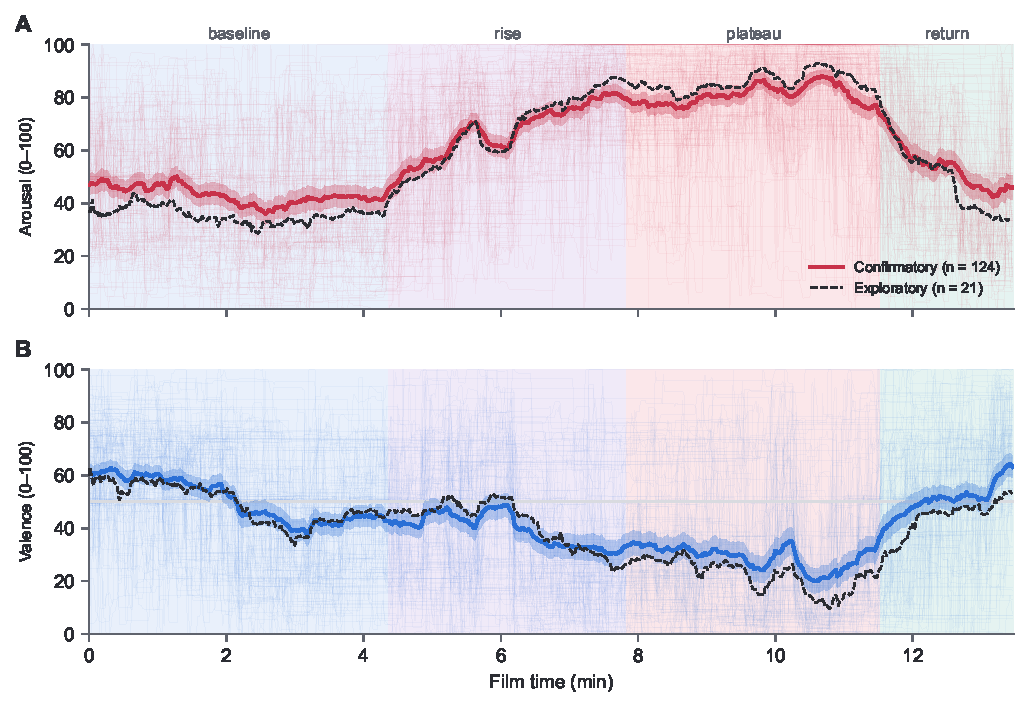
\includegraphics[width=\textwidth]{figure1.pdf}
\figurenote{(A) Arousal (0~=~low, 100~=~high) and (B) valence (0~=~unpleasant, 50~=~neutral, 100~=~pleasant), rated
continuously and resampled to 1~Hz. Thin lines are individual participants of the confirmatory sample; the thick line
is the group mean with its 95\% confidence interval ($N$~=~\val{n_primary}); the dashed line is the group mean of the
exploratory sample ($n$~=~\val{n_exploratory}). Shading marks the four preregistered segments, estimated from
group-mean arousal in the exploratory sample. The segment names are descriptive labels; the opening segment is called
baseline in the preregistration.}
\end{figure}

\begin{figure}[tbp]
\caption{Somatic Anxiety Before and After the Film}
\label{fig:sticsa}
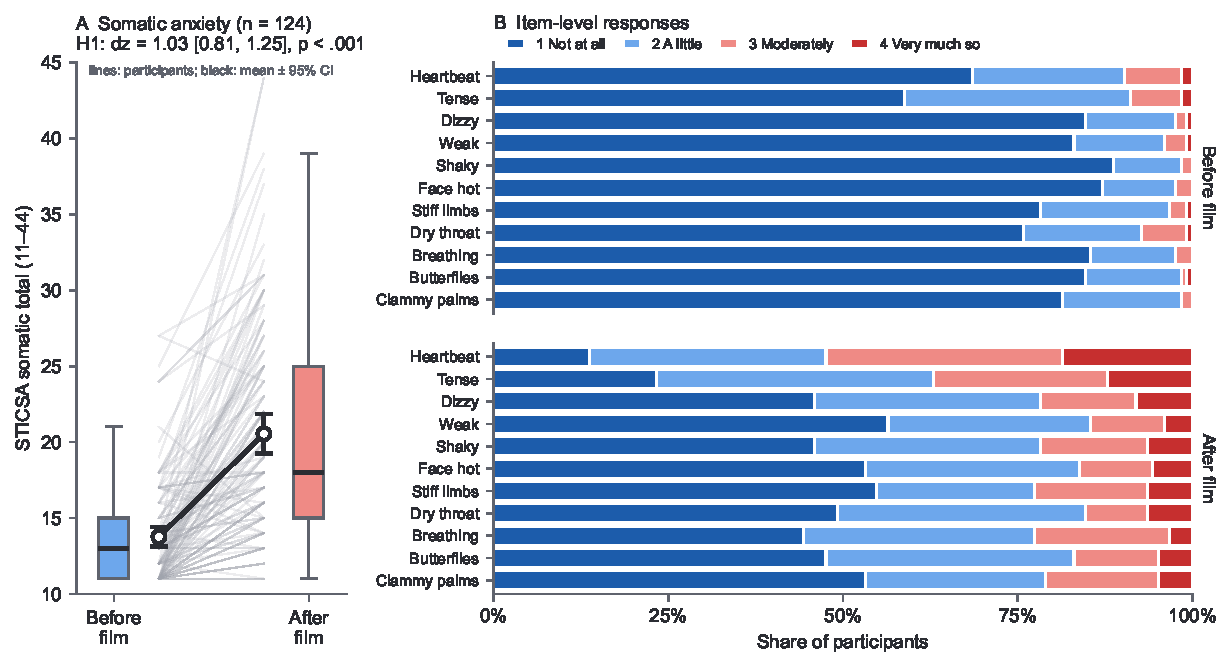
\includegraphics[width=\textwidth]{figure2.pdf}
\figurenote{(A) STICSA somatic totals (11--44) before and after the film in the confirmatory sample
($N$~=~\val{n_primary}). Grey lines connect each participant's scores; boxes show medians and interquartile ranges;
the black line shows means with 95\% confidence intervals. (B) Share of participants giving each answer (1~=~not at all
to 4~=~very much so) to the eleven somatic items before (top) and after (bottom) the film; items are ordered as in the
questionnaire.}
\end{figure}

\end{document}
